\chapter{Introduction}


\section{Social relevance}
Atrial Fibrillation is the most common type of cardiac arrhythmia.
Thousands of heart failures could be prevented by proper treatment if early signs were diagnosed in time.
Over the years medical equipment advanced by involving some sort of artificial intelligence.
We don't have to go far, probably every gas station in the area has a semi-automatic defibrillator, that has a sensor built in which recognizes whether the patient needs to be shocked or not --- to prevent unnecessary reanimation.
The basic idea is to relieve overwhelmed doctors by recognizing invariant patterns in the specific cases.
These patterns are taught in medical universities, and fine-tuned during years of practice --- but turns out that volunteering cardiologists can submit their knowledge base to engineers who in return will automatize at least the trivial process to support the better treatment.
In order to assist in the diagnosis, and make predictions based on previous cases we utilize Machine Learning techniques to combine professional knowledge and neural networks to achieve the lowest error rate on a classifying task.
%
% \section{Biological background}
% Atrial fibrillation is evoked

\section{The real challenge}
This year the PhysioNet Challenge~\cite{noauthor_af_nodate} is simple, a set of single lead ECG samples labeled by a team of cardiologists is provided. The labels are the following: \textit{noisy, normal, atrium fibrillation, other}. The task is to develop a method that is able to classify from an unseen prerecorded sample.
At first sight the initial conditions are very encouraging, but soon after the first check of the training files it turns out that only a limited number of samples are given, exactly 8528 samples, the dataset has a strongly imbalanced distribution between classes.

Also as it was revealed during the last weeks, the ground truth had several errors, misleading the training process.
We had several discussions in the early phase of development with professionals about possible classification errors, that even were trivial to us~\ref{fig:trivial}. Many suggestions were committed by the competitors, and as a result the organizers released an updated label reference.
The difference depicted in details on Figure ~\ref{fig:pie}.
\begin{figure}[h!]
  \centering
  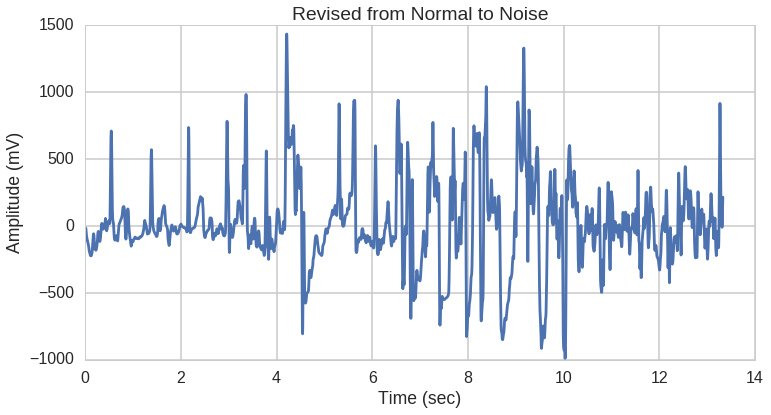
\includegraphics[width=\textwidth]{trivial}
  \caption{The depicted ECG signal was originally classified as a \textit{normal} sample, later revised to \textit{noisy}.}
  \label{fig:trivial}
  \vspace*{\floatsep}

  \centering
  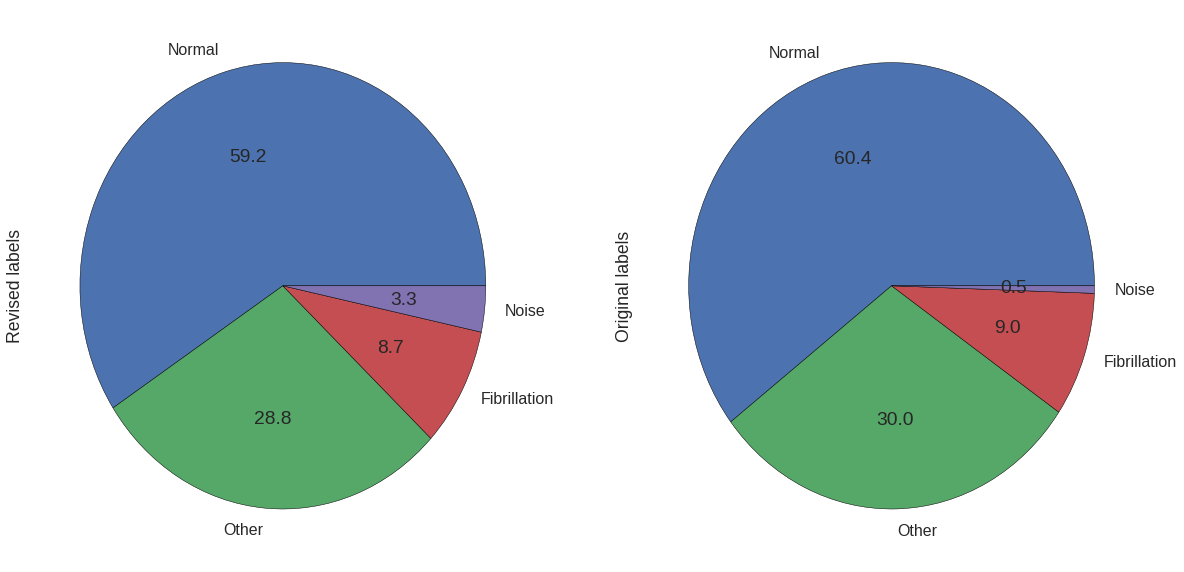
\includegraphics[width=\textwidth]{pie}
  \caption{The differences between the original (left) and the revised (right) ground truth labels. According to the latest update, the noise class is still underrepresented, and still it is very likely that any model trying to discriminate noisy samples will be too simple to classify them all correctly, or with larger capacity will be over-fitted.}
  \label{fig:pie}
\end{figure}
